\documentclass[10pt]{article}
% We could also do
% \documentclass[10pt, twoside]{article}
% which shifts everything slightly to the
% side which makes it easier to read if
% it's all stapled together. 
\usepackage[doublespacing]{setspace}
\usepackage{mathtools}
\usepackage{array}
\usepackage{booktabs}
\usepackage{float}
\usepackage{amsmath}
\usepackage{amsfonts}
\usepackage{amssymb}
\usepackage{amsthm}
\usepackage{enumitem}
\usepackage{graphicx}
\usepackage{xcolor}
\graphicspath{{.}}
\title{Optimizing the Robotics Closet}
\author{Sasha Krassovsky, John Lim, Andrey Ryabtsev}
\begin{document}
\maketitle
\pagebreak

\section{Introduction}
The Husky Robotics team is a team of both undergraduate and graduate students
from UW building a Mars rover to compete in the University Rover Challenge.
The rover must perform a variety of tasks, such as autonomous navigation, soil
collection, and typing on a keyboard with a robotic arm. The team is divided
into subsystems: Chassis, Arm, Science, Electronics, Software, and Manufacturing.
The subsystems work independently but collaborate to create the robot. Given
all these tasks and the relatively short amount of time given to build out the
functionality, efficiency is key when it comes to the build process.
\par
The robotics team has only a small closet in the Mechanical Engineering Building.
The closet stores the robot along with all of the tools, electronics, sheet metal,
carbon fiber, and plastics that go into building the robot. Each item belongs to
one of the subsystems, and is usually stored near other items belonging to that
subsystem. Unfortunately, the robotics closet is not particularly organized, and
members often spend on the order of 10 minutes looking for the thing they needed.
Our goal is to find a reorganization plan for the items in the closet such that
expected duration of each closet visit is minimized and items belonging to the
same subsystem are in the same connected component on the shelves.
\par
The closet has two shelves, one on each side. One side stores items in
uniformly-sized boxes while the other side has several other classes of items,
such as soldering irons, and boxes of various sizes. The rover is stored in
the middle of the room on a big cart. Behind it is the robotic arm and the
science station. In the back are the sheet metal, various metallic cylinders,
wood, and rolls of carbon fiber. By examining the frequencies of retrieval
by each team and treating the closet as a grid, we should be able to produce
a better layout of the closet.

\begin{center}
  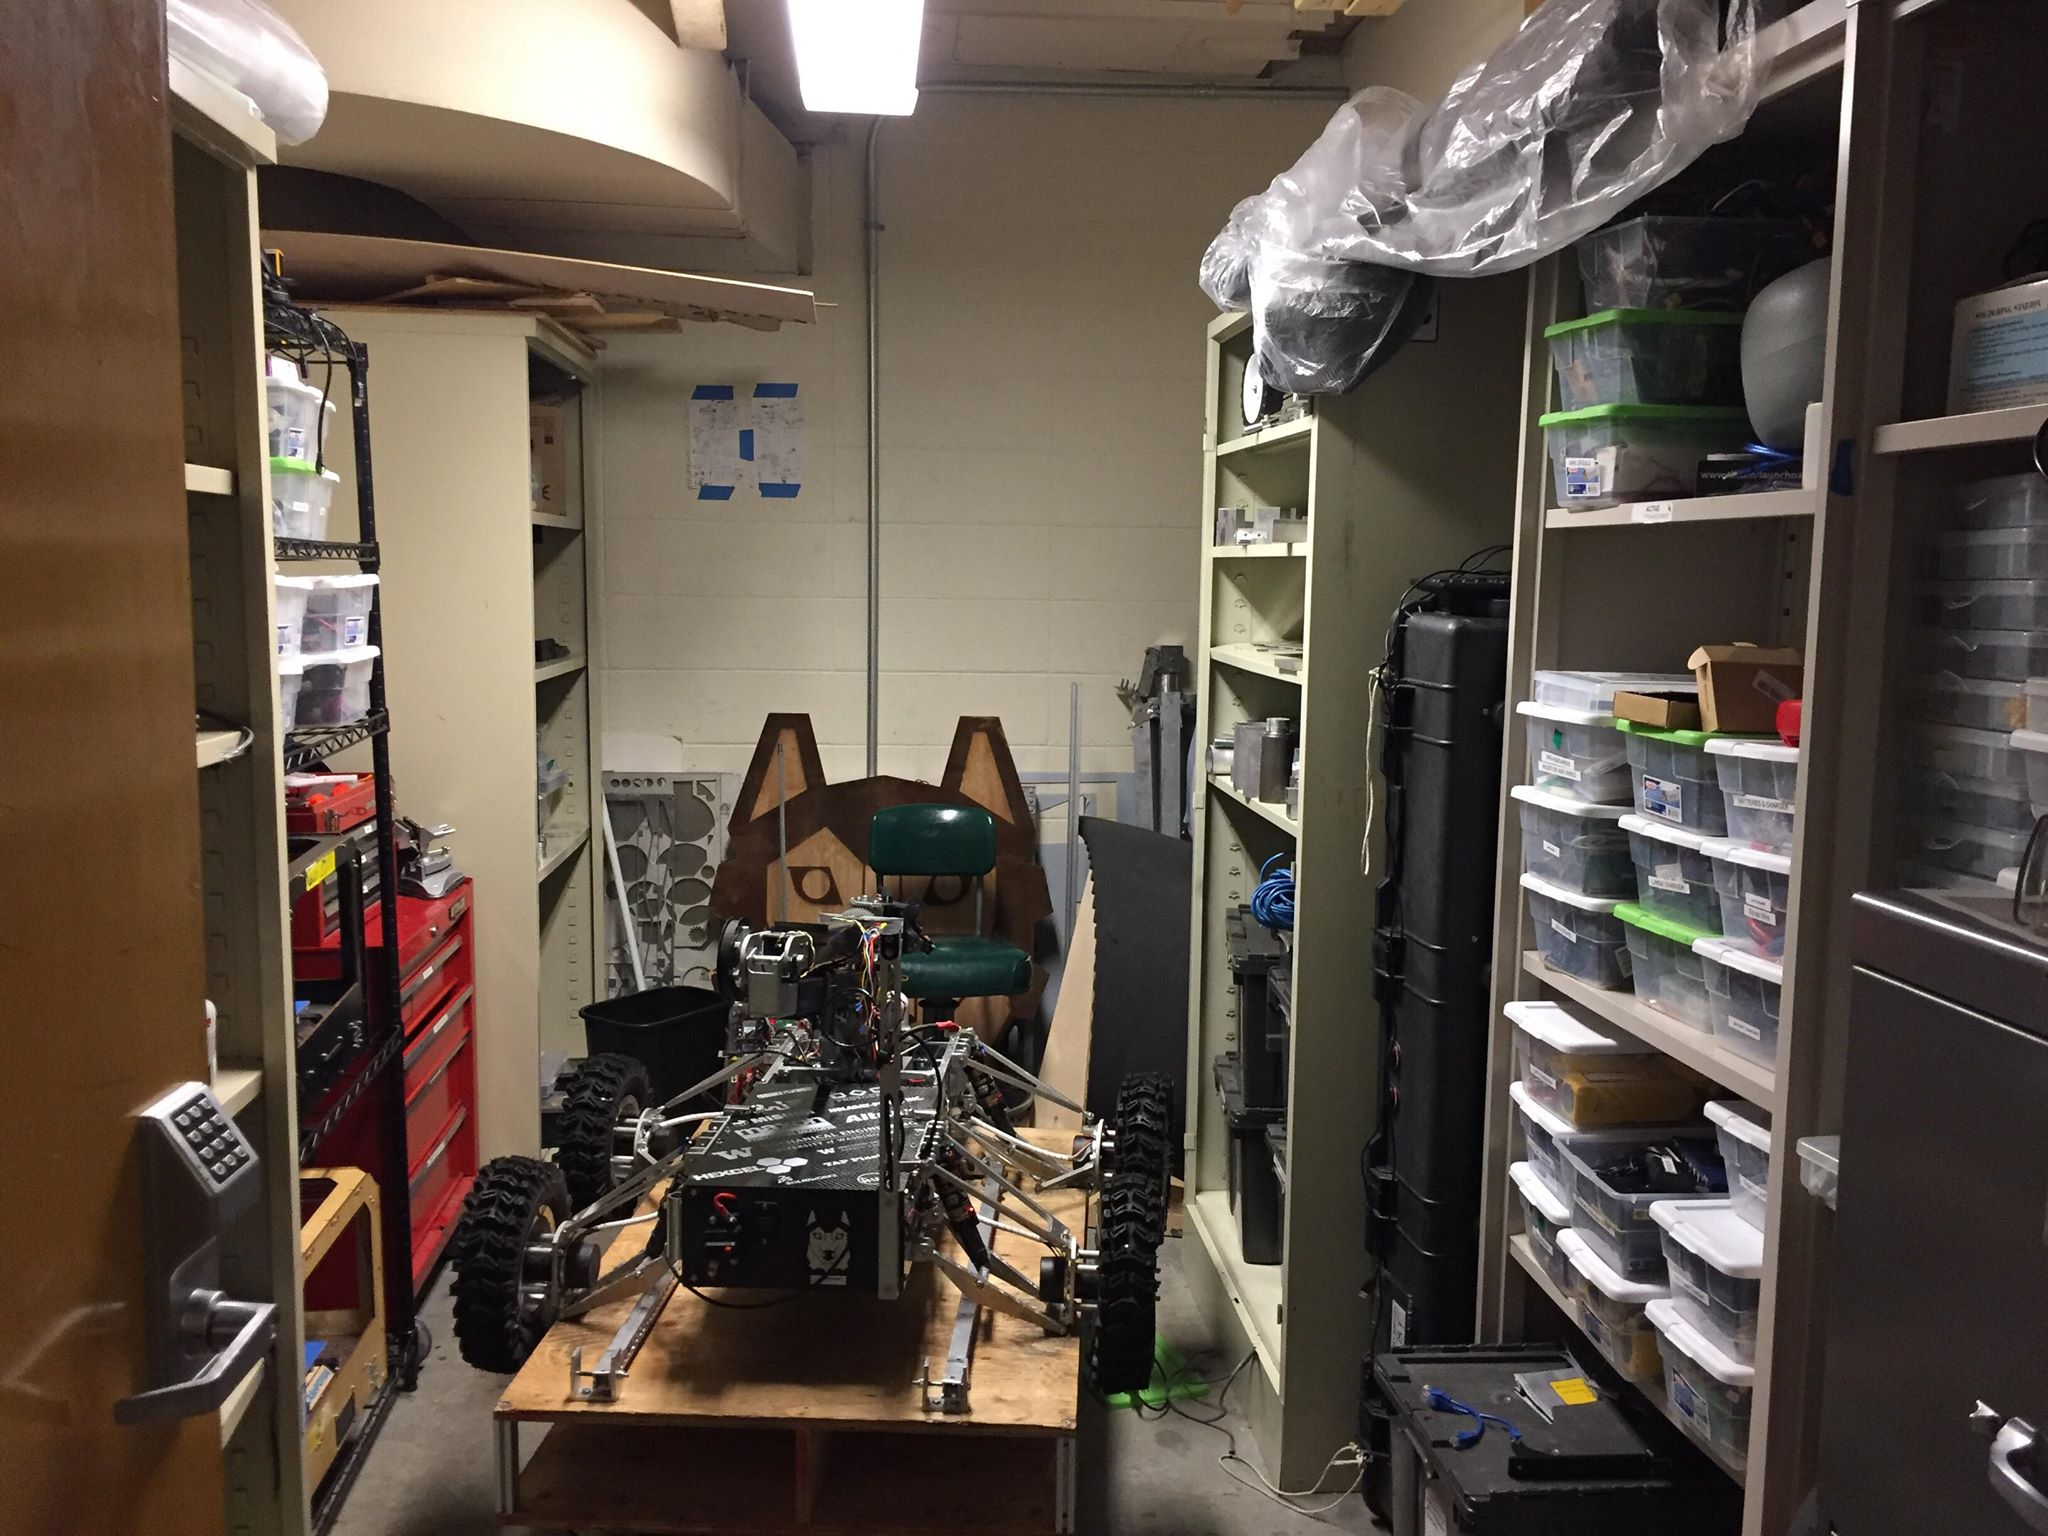
\includegraphics[scale=0.15]{closet.jpg} \\
  The robotics closet before optimization. 
\end{center}

\section{Related Work}
Deepesh Singh's \emph{A Beginner’s guide to Shelf Space Optimization using Linear Programming}
explains an integer programming formulation for finding the optimal layout of a store
that maximizes sales. The guide organizes the store into several racks, each with
a certain number of shelves. One key assumption is that only one product can fit
on a rack. The model uses a table showing how many sales are generated by each item
depending on which rack it is placed. The objective function is then the profit
generated by a given arrangement. Arrangements are represented by a matrix, with
each $a_{ij}$ representing whether product $j$ is on shelf $i$. If it is, the
$a_{ij}$ is $1$ and $0$ otherwise. The guide shows how to maximize this profit function.
Although this approach is a good start, our problem differs in several ways: we can
fit more than one box on each shelf, and our goal is to minimize time of retrieval
rather than maximize profits.

\textbf{\color{red} TODO: More related work}

\section{Assumptions}
Most items in the robotics closet are in boxes. As a result, we assume that all
items are rectangular prisms. Although items such as the chemicals or soldering irons
are not strictly rectangle-shaped, it would be strange for another item reached into
the empty areas of the items' bounding boxes. Taking advantage of this, we approximate
all items as being rectangular prisms, and measure their bounding boxes.
\par
\section{Model}

\end{document}
